\section{Binary Classification Experiment Results}


\section{Multi-Class Classification Experiment Results}
\begin{figure}[h]
	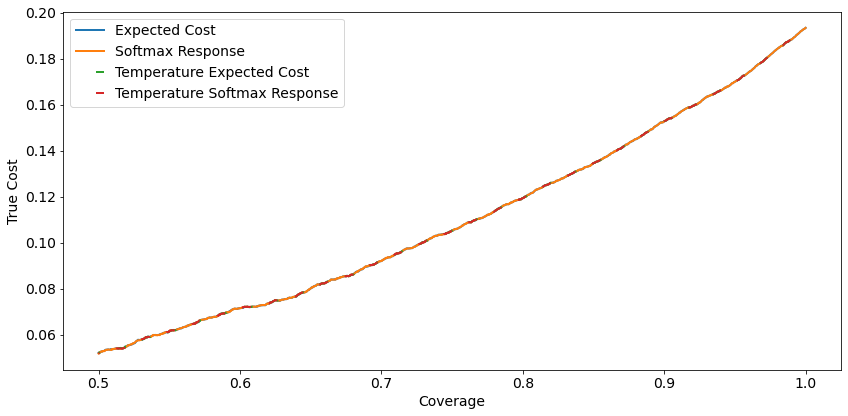
\includegraphics[width=\textwidth]{images/multi-class/cnn-sym.png}
	\caption{Experiments using a standard CNN with symmetrical costs.}
\end{figure}

\begin{figure}[h]
	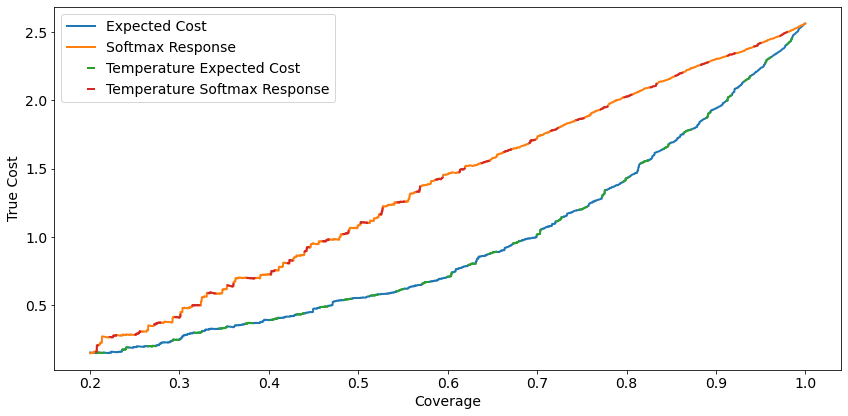
\includegraphics[width=\textwidth]{images/multi-class/cnn-asym.png}
	\caption{Experiments using a standard CNN with asymmetrical costs.}
\end{figure}

\begin{figure}[h]
	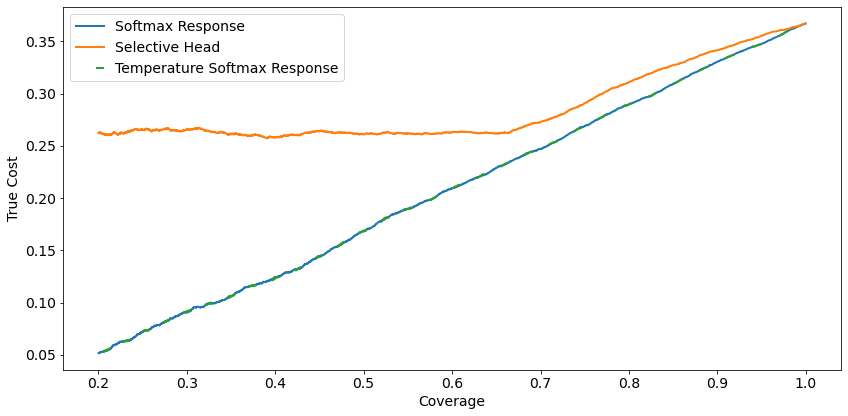
\includegraphics[width=\textwidth]{images/multi-class/sn0.7-sym.png}
	\caption{Experiments using a SelectiveNet model with a target coverage of 0.7 with symmetrical costs.}
\end{figure}

\begin{figure}[h]
	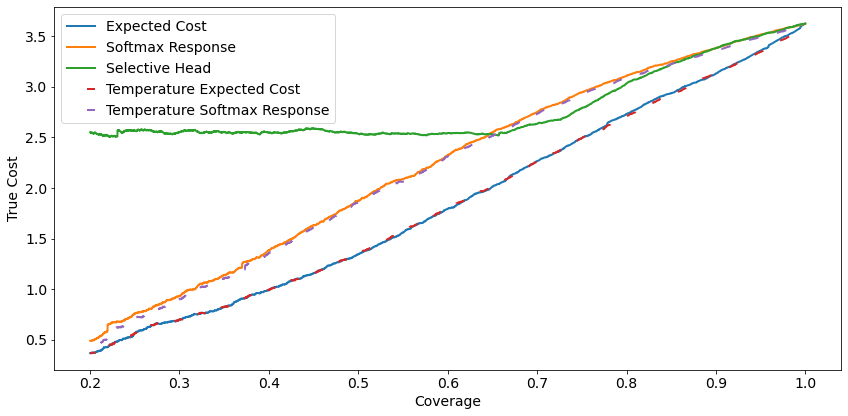
\includegraphics[width=\textwidth]{images/multi-class/sn0.7-asym.png}
	\caption{Experiments using a SelectiveNet model with a target coverage of 0.7 with asymmetrical costs.}
\end{figure}

\begin{figure}[h]
	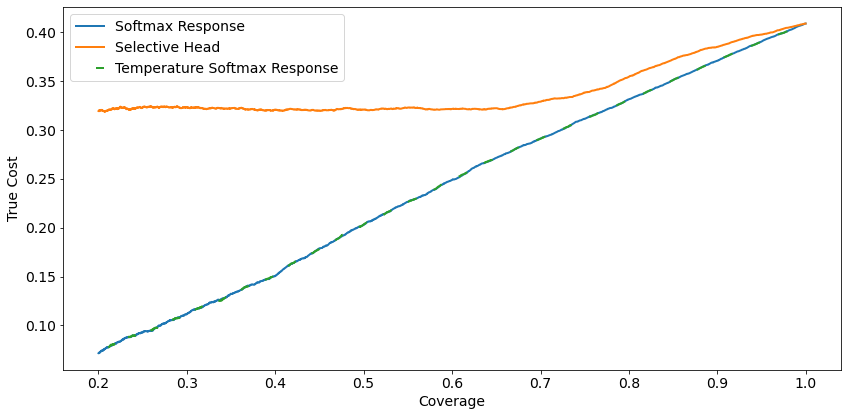
\includegraphics[width=\textwidth]{images/multi-class/sn0.75-sym.png}
	\caption{Experiments using a SelectiveNet model with a target coverage of 0.75 with symmetrical costs.}
\end{figure}

\begin{figure}[h]
	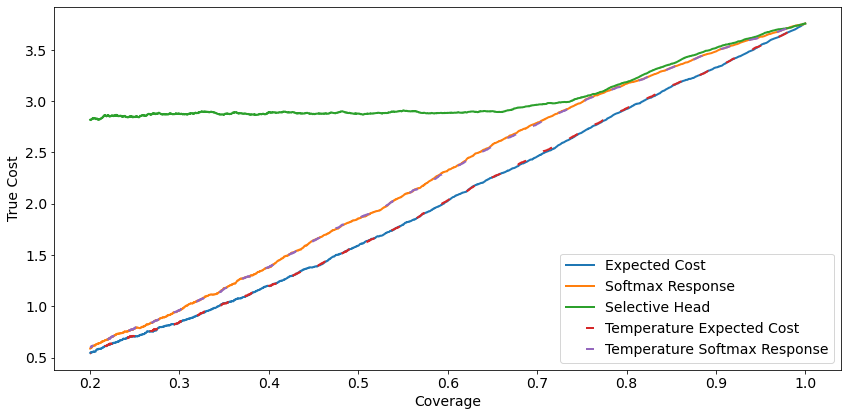
\includegraphics[width=\textwidth]{images/multi-class/sn0.75-asym.png}
	\caption{Experiments using a SelectiveNet model with a target coverage of 0.75 with asymmetrical costs.}
\end{figure}

\begin{figure}[h]
	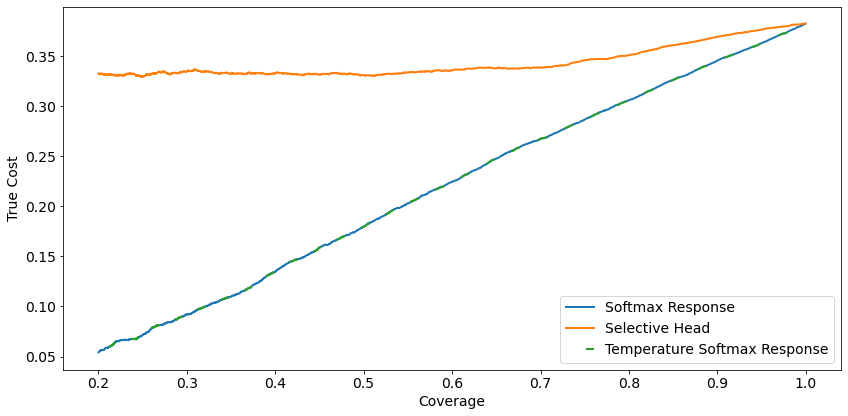
\includegraphics[width=\textwidth]{images/multi-class/sn0.8-sym.png}
	\caption{Experiments using a SelectiveNet model with a target coverage of 0.8 with symmetrical costs.}
\end{figure}

\begin{figure}[h]
	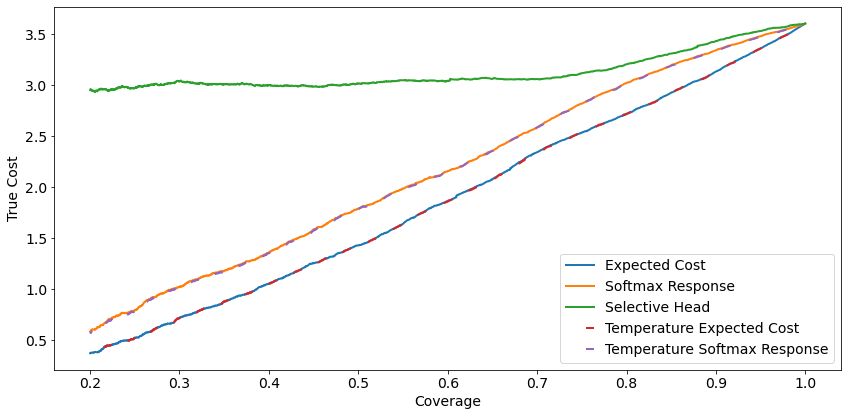
\includegraphics[width=\textwidth]{images/multi-class/sn0.8-asym.png}
	\caption{Experiments using a SelectiveNet model with a target coverage of 0.8 with asymmetrical costs.}
\end{figure}

\begin{figure}[h]
	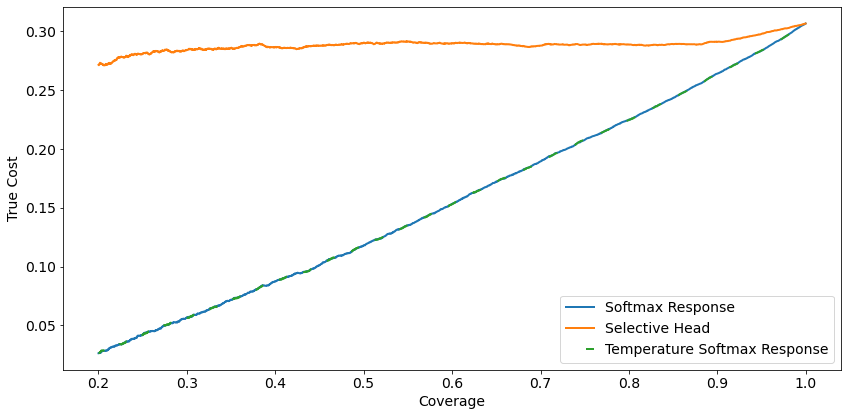
\includegraphics[width=\textwidth]{images/multi-class/sn0.85-sym.png}
	\caption{Experiments using a SelectiveNet model with a target coverage of 0.85 with symmetrical costs.}
\end{figure}

\begin{figure}[h]
	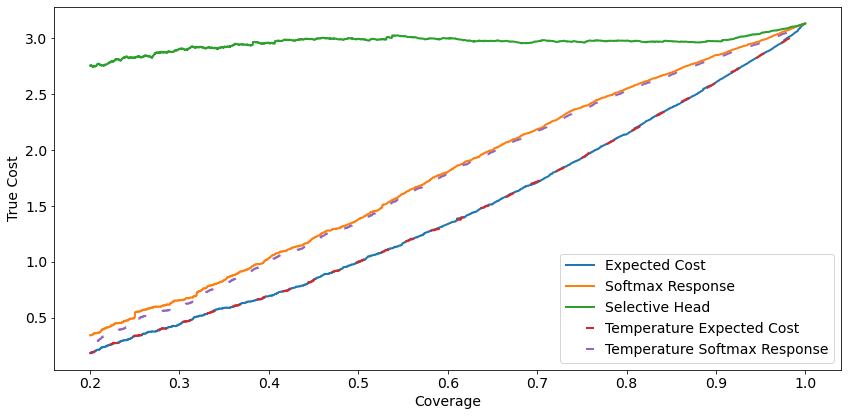
\includegraphics[width=\textwidth]{images/multi-class/sn0.85-asym.png}
	\caption{Experiments using a SelectiveNet model with a target coverage of 0.85 with asymmetrical costs.}
\end{figure}

\begin{figure}[h]
	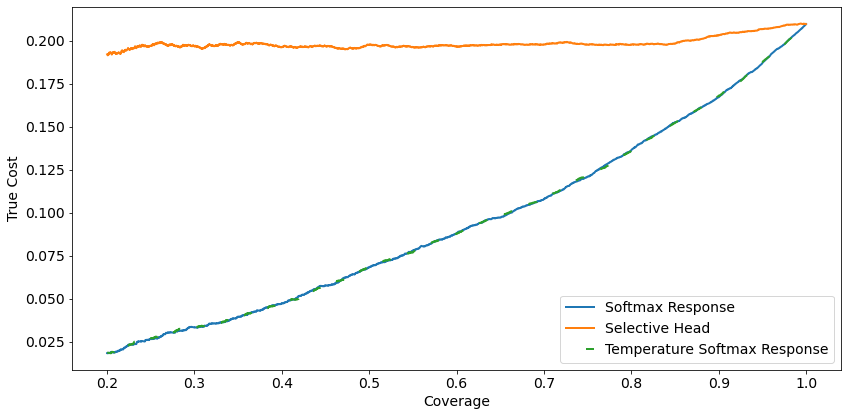
\includegraphics[width=\textwidth]{images/multi-class/sn0.9-sym.png}
	\caption{Experiments using a SelectiveNet model with a target coverage of 0.9 with symmetrical costs.}
\end{figure}

\begin{figure}[h]
	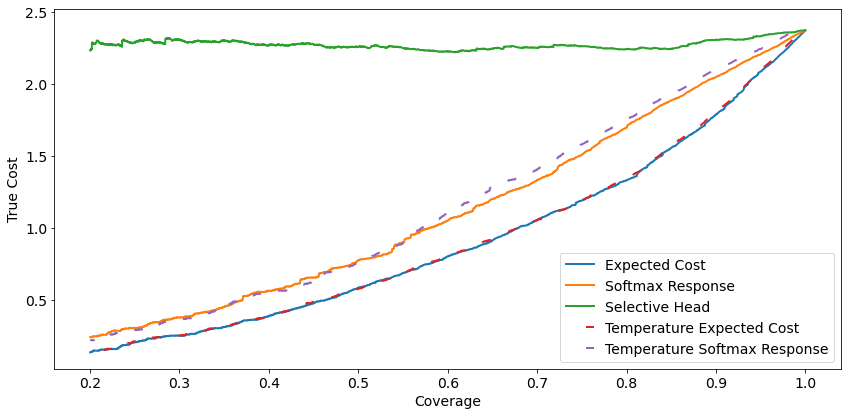
\includegraphics[width=\textwidth]{images/multi-class/sn0.9-asym.png}
	\caption{Experiments using a SelectiveNet model with a target coverage of 0.9 with asymmetrical costs.}
\end{figure}

\begin{figure}[h]
	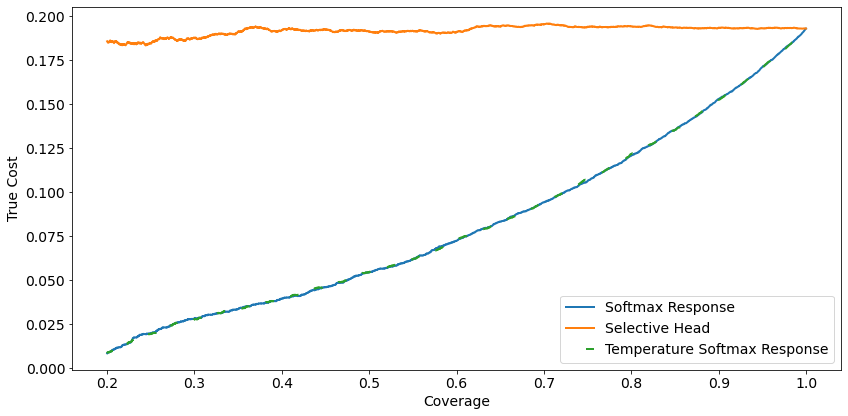
\includegraphics[width=\textwidth]{images/multi-class/sn0.95-sym.png}
	\caption{Experiments using a SelectiveNet model with a target coverage of 0.95 with symmetrical costs.}
\end{figure}

\begin{figure}[h]
	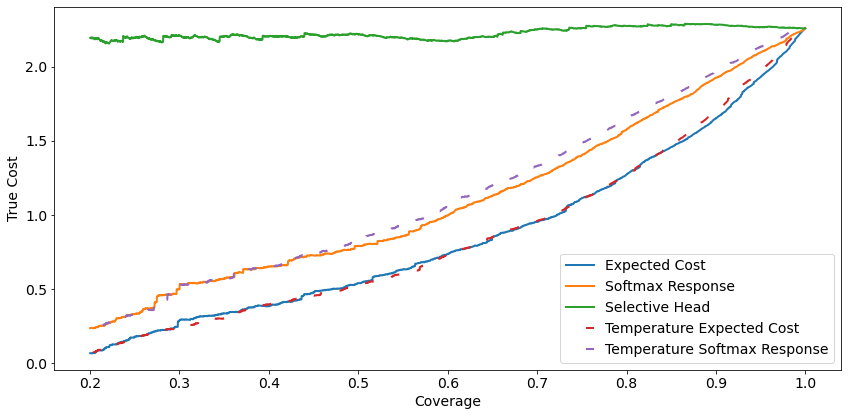
\includegraphics[width=\textwidth]{images/multi-class/sn0.95-asym.png}
	\caption{Experiments using a SelectiveNet model with a target coverage of 0.95 with asymmetrical costs.}
\end{figure}

\begin{figure}[h]
	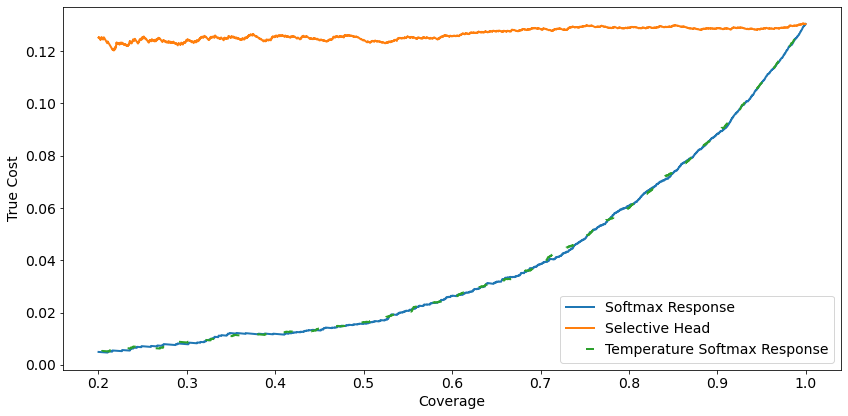
\includegraphics[width=\textwidth]{images/multi-class/sn1.0-sym.png}
	\caption{Experiments using a SelectiveNet model with a target coverage of 1.0 with symmetrical costs.}
\end{figure}

\begin{figure}[h]
	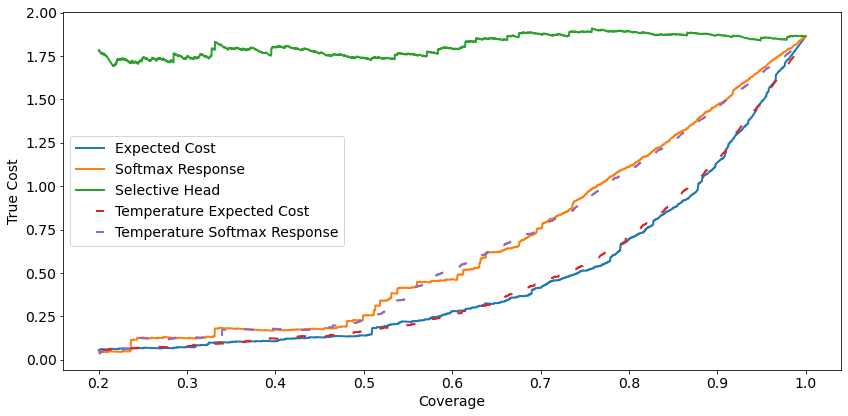
\includegraphics[width=\textwidth]{images/multi-class/sn1.0-asym.png}
	\caption{Experiments using a SelectiveNet model with a target coverage of 1.0 with asymmetrical costs.}
\end{figure}

\begin{figure}[h]
	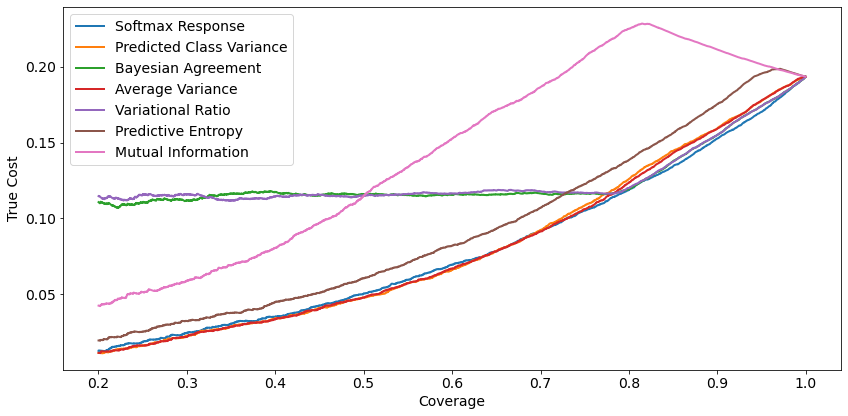
\includegraphics[width=\textwidth]{images/multi-class/mc-dropout-sym.png}
	\caption{Experiments using a Bayesian model with Monte Carlo Dropout with symmetrical costs.}
\end{figure}

\begin{figure}[h]
	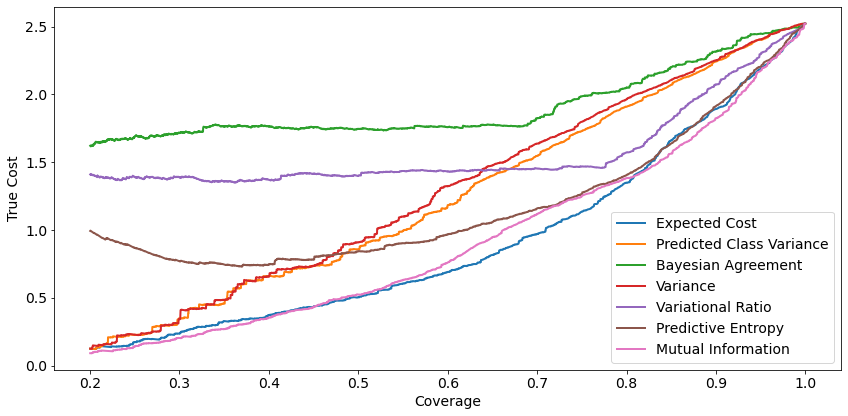
\includegraphics[width=\textwidth]{images/multi-class/mc-dropout-asym.png}
	\caption{Experiments using a Bayesian model with Monte Carlo Dropout with asymmetrical costs.}
\end{figure}

\begin{figure}[h]
	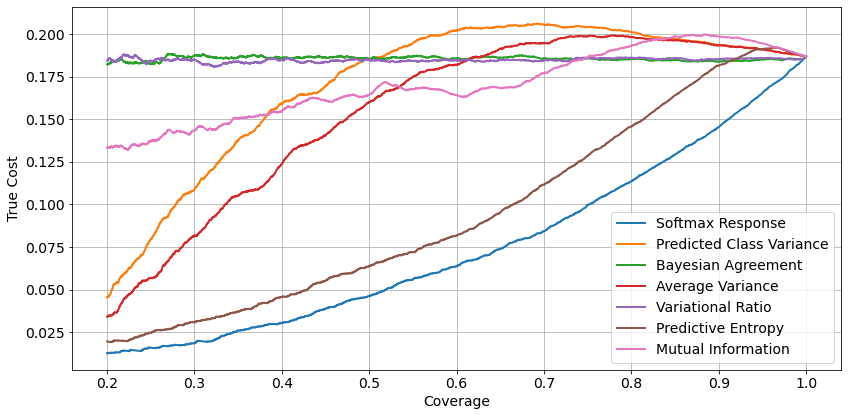
\includegraphics[width=\textwidth]{images/multi-class/bbb-sym.png}
	\caption{Experiments using a Bayesian model trained using Bayes-by-Backprop with asymmetrical costs.}
\end{figure}

\begin{figure}[h]
	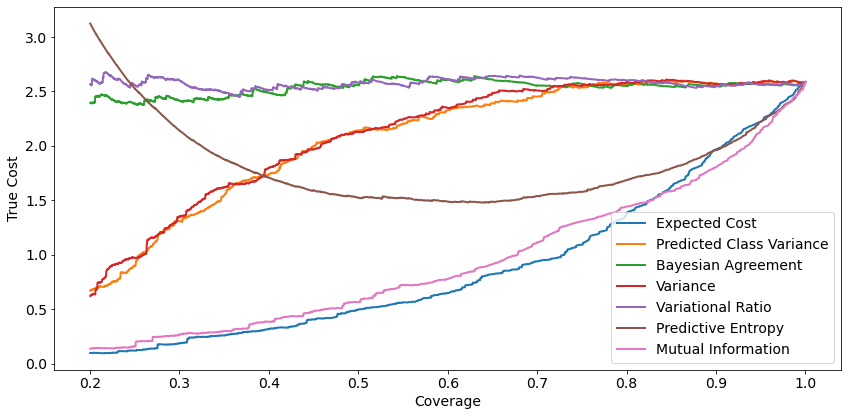
\includegraphics[width=\textwidth]{images/multi-class/bbb-asym.png}
	\caption{Experiments using a Bayesian model trained using Bayes-by-Backprop with asymmetrical costs.}
\end{figure}


\begin{figure}[h]
	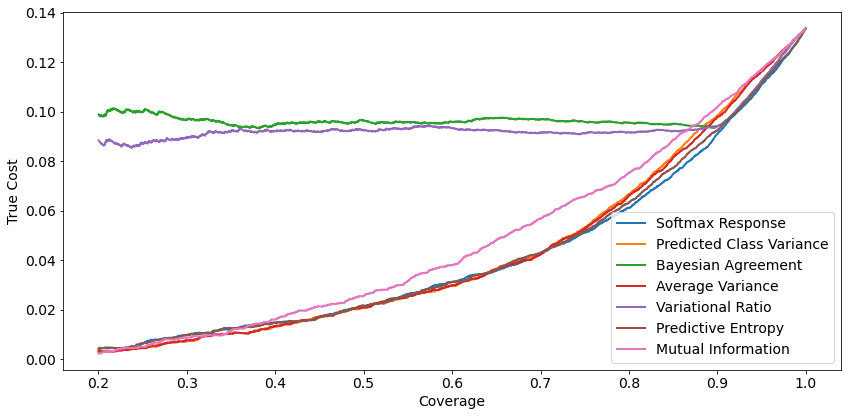
\includegraphics[width=\textwidth]{images/multi-class/laplace-sym.png}
	\caption{Experiments using a Bayesian model trained using Laplace Approximation with symmetrical costs.}
\end{figure}

\begin{figure}[h]
	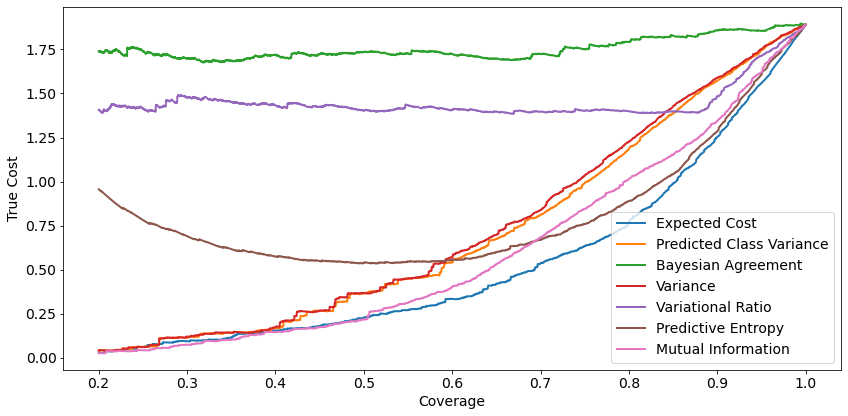
\includegraphics[width=\textwidth]{images/multi-class/laplace-asym.png}
	\caption{Experiments using a Bayesian model trained using Laplace Approximation with asymmetrical costs.}
\end{figure}